\documentclass[aps,prl,superscriptaddress,groupedaddress]{revtex4}
\usepackage{graphicx}  % needed for figures
\usepackage{dcolumn}   % needed for some tables
\usepackage{bm}        % for math
\usepackage{amssymb,amsmath} % for math
\usepackage{tikz} % for drawing
\usepackage{subfig} % for subfigure
\usetikzlibrary{calc} % for tikz calculations
\usetikzlibrary{arrows,decorations.markings} % make arrow head bigger
\usepackage{array} % for changing table height
\usepackage{comment}
\usepackage[bookmarks]{hyperref}

% avoids incorrect hyphenation, added Nov/08 by SSR
\hyphenation{ALPGEN}
\hyphenation{EVTGEN}
\hyphenation{PYTHIA}

\begin{document}

\widetext
\title{Accurate Predictions of Ionization and Atomization Energies without the Born-Oppenheimer Approximation}
\author{Yubo Yang}
\author{Ilkka Kyl\"{a}np\"{a}\"{a}}
\author{Norm M. Tubman}
\affiliation{Department of Physics, University of Illinois, Urbana, Illinois 61801 USA}
\author{Jaron T. Krogel}
\affiliation{Materials Science \& Technology Division, Oak Ridge National Laboratory, Oak Ridge, TN 37831}
\author{Sharon Hammes-Schiffer}
\affiliation{Department of Chemistry, University of Illinois, Urbana, Illinois 61801 USA}
\author{David M. Ceperley}
\affiliation{Department of Physics, University of Illinois, Urbana, Illinois 61801 USA}
\date{\today}

\begin{abstract}
We obtained ground-state energies of a range of small atoms and molecules with Fixed-Node Diffusion Monte Carlo (FN-DMC) to an accuracy of $0.01\text{mHa}$ ($0.27\text{meV}$), treating both electrons and ions as quantum particles. We used "dragged node approximation" developed by Tubman et. al to construct the trial wavefunction without the adiabatic assumption. For each system, we optimized an all-electron trial wavefunction generated by quantum chemistry methods and used it to construct an all-electron-ion wavefunction. It is then used in FN-DMC to obtain the ground-state energy of said system. We found the ionization energies of first row atoms to be identical with or without the adiabatic assumption, whereas the atomization energies of simple hydrides to change by as much as 6.2\%. The non-adiabatic results are in better agreement with the best available quantum chemistry literature in all tested hydrides.
\end{abstract}
\maketitle

\section{Introduction}
Under the adiabatic assumption, often also referred to as the Born-Oppenheimer (BO) approximation \cite{BO}, the full atomic/molecular Hamiltonian is divided up into an electron component and an ion component. The electron problem is solved by "clamping" the ions to their equilibrium positions. Then, the ion problem is solved using the equilibrium electron distribution as an effective potential energy surface. This assumption is based on the fact that protons are roughly 1836 times as heavy as electrons and thus ions, being heavier than protons, move much more slowly than electrons, allowing the electrons to relax instantaneously and adiabatically to their equilibrium states as the ions move around. The BO approximation is excellent in most cases, but recent advances suggest one might be missing important physics by adopting this approximation in certain cases. For example the prediction of ground state structure of atomic hydrogen \cite{Ceperley_1987,Natoli_1993,Natoli_1995}, the dissociation of hydrogen at finite temperature \cite{Mazzola_FiniteT} and photon coupled electron transfer (PCET) in phenoxyl-phenol \cite{Sirjoosingh_PCET} were only possible due to the inclusion of non-adiabatic effects.

While there have been many cases in the literature where non-adiabatic effects were included for atomic and molecular systems, they tend to require a great deal of computational as well as human effort. One approach is to add corrections to a basic coupled cluster theory to produce highly accurate ground state energies for atoms and molecules\cite{Feller_Corrections}. In such an approach, a frozen-core coupled cluster singles and doubles (FC-CCSD) \cite{Purvis_CCSD} calculation serves as a first approximation for the ground-state energies. Then a series of corrections including core/valance, spin-orbit coupling, higher order correlation, zero point motion, diagonal Born-Oppenheimer and scalar relativistic effects are introduced. Each correction involves a non-trivial and often costly calculation and extrapolation formulae are sometimes needed to take the result to the complete basis set limit. This method produces highly accurate expectation values, but contains uncontrolled errors that have to be estimated either empirically or analyzed on a molecule-by-molecule basis \cite{Feller_Error}. The addition of uncertainties in each correction also contributes to a rather large error bar, making it difficult to obtain a small confidence interval with this method. Another approach in a more recent development is to use the explicitly correlated Gaussian (ECG) basis \cite{Adamowicz_ECG,Mitroy_ECG}. This approach is capable of calculating the ground-state energies of small molecules to an incredibly high accuracy. Unfortunately, the current implementation of ECG cannot be applied to moderately-sized systems due to factorial scaling with the number of identical particles \cite{Bubin_BH_noBO}. Other methods with less aggressive scaling include nuclear-electronic orbital (NEO) Hatree-Fock (HF) \cite{Sharon_NEO}, NEO explicitly correlated HF (NEO-ECHF) \cite{Sharon_NEOX,Sharon_NEOX1,Sharon_NEOX2}, path integral Monte Carlo \cite{Ilkka_Path,Ilkka_Path1,Ilkka_Path2} and multicomponent density functional theory \cite{Sharon_NEO-DFT,Sharon_NEO-DFT1,Sharon_NEO-DFT2,Sharon_NEO-DFT3,Gross_NEO-DFT,Gross_NEO-DFT1}. While these methods can be applied to larger systems, it would be difficult to deliver the same kind of accuracy that ECG offers without significant development. In this paper, we would like to demonstrate that, with simple modifications \cite{Tubman_ECG}, the fixed-node diffusion Monte Carlo (FN-DMC) algorithm is capable of producing results on par with and even better than the most sophisticated quantum chemistry methods for systems as small as BH.

\section{Method}
\subsection{Fixed-Node Diffusion Monte Carlo (FN-DMC)}
FN-DMC is a simple but powerful projector method that evolves the exact Hamiltonian in imaginary time and projects out the ground-state wavefunction in the infinite time limit. 

Quantum Monte Carlo(QMC) methods are capable of producing highly accurate ground state wavefunctions for atomic and molecular systems if a good initial guess is given. Due to the introduction of linear optimization method by Nightingale et. al.\cite{Nightingale_Linear} and Umrigar et. al.\cite{Umrigar_Linear}, one can systematically improve the wave function ansatz generated by quantum chemistry calculations to obtain high quality wave functions for atoms and molecules as was done by Brown\cite{Brown_Bench} and Toulouse\cite{Toulouse_Bench}.  This assumption allows us to partially decouple the electron and ion problems \cite{McMahon_Review}. In almost all previous QMC calculations, the authors worked within the adiabatic assumption where the motions of the ions are assumed to be decoupled from those of the electrons. However, such an assumption is not fundamentally required by QMC. It's inclusion is mostly due to a lack of mean field theories that include non-adiabatic effects. Although there is significant effort in the quantum chemistry community to develop such methodology \cite{Sharon_NEO,Sharon_NEO1}, until a standardized package is developed we will have to rely on modification of the QMC algorithm itself to include non-adiabatic effects. To this end, Tubman et. al. \cite{Tubman_ECG} developed a straightforward algorithm to construct a high quality all-electron-ion wavefunction from an optimized all-electron wavefunction.
\subsection{Electron Wavefunction and Optimization}
We followed the basic strategies of Umrigar et. al.\cite{Umrigar_Alleviation,Toulouse_Bench} and Needs et. al. \cite{Brown_Bench,Seth_Bench} in generating our all-electron wavefunctions. The initial guess for the wavefunction is generated from Complete Active Space Self-Consistent Field (CASSCF) \cite{Chaban_MCSCF,Szabo} calculation using the quantum chemistry package GAMESS-US\cite{GAMESS}. The optimized orbitals are then used in a Second Order Configuration Interaction (SOCI) calculation to generate a series of Configuration State Functions (CSF). This process is described in more detail in \cite{Clark_Bench}. The multi-CSF expansion of the wavefunction generated by GAMESS can be expressed in the following form
\begin{align}
\Psi_{SOCI}(\vec{r})=\sum\limits_{i=1}^{N_{CSF}}\alpha_i\phi_i(\vec{r}) \label{eq:psi_gms}
\end{align}
where $\vec{r}$ refers to the spacial coordinates of all the electrons. $\alpha_i$ and $\phi_i(\vec{r})$ are the coefficients and CSF generated from SOCI respectively. We used the cc-pV5Z basis for all the atomic systems but switched to Roos Augmented Triple Zeta ANO basis for molecular systems due to GAMESS's limited ability to handle a large number of basis elements. Both basis sets are taken from Basis Set Exchange \cite{BSE}.

A Jastrow factor $J(\vec{r},\vec{\beta})$, in the form of a B-spline with values $\vec{\beta}$ on a linear grid, is then added to the wave function to correlate electron motion and smooth out the divergence in the local energy near the ions by imposing the cusp condition \cite{Kato}. Our Jastrow factor contains electron-electron, electron-nucleus and electron-electron-nucleus terms. The actually wave function being optimized is then
\begin{align}
\Psi_e(\vec{r})=e^{J(\vec{r},\vec{\beta})}\sum\limits_{i=1}^{N_{CSF}}\alpha_i\phi_i(\vec{r})\label{eq:psie}
\end{align}
The optimization is performed using linear optimization with QMCPACK\cite{QMCPACK}. We optimized the CSF and Jastrow coefficients ($\vec{\alpha}$,$\vec{\beta}$) simultaneously with a cost function consisting of $50\%$ average local energy and $50\%$ reweighted variance. We found this choice of cost function to produce slightly better wavefunctions than a highly biased one ($90\%$ energy+$10\%$ variance or $10\%$ energy+$90\%$ variance). Although the differences are small and are likely insignificant at the DMC level.

For all of the systems we studied, the SOCI ground state CSF $\phi_0(\vec{r})$ always dominates the expansion (with $\alpha_0>.95$). Nevertheless, we include all CSFs with coefficients bigger than some cutoff $\epsilon$ to lend reasonable flexibility to the wavefunction during optimization. The choice of $\epsilon$ is somewhat arbitrary. We wish to included as many CSFs as possible to maximize the flexibility of the wave function. However, the inclusion of too many CSFs with small expansion coefficients introduce unnecessary noise into the system and require a large number of samples in the optimization loop to reach our desired accuracy. Therefore, we have chosen $\epsilon$ to restrict the number of CSFs in the wave function to be $\sim$1000 to maintain a balance between the flexibility and the cost of optimization. In most of our systems, this criteria results in an $\epsilon$ of $0.001\sim0.0001$ and the sum of coefficients squared of the included CSFs $\sum\limits_{i}a_i^2 > 0.999$ in all cases.

\subsection{Electron-Ion Wavefunction}
Once a satisfactory electron wave function has been obtained, we construct the electron-ion wave function using the following an ansatz suggested by Tubman et. al.\cite{Tubman_ECG}
\begin{align}
\Psi_{ei}(\vec{r},\vec{R})=\psi_I(\vec{R})\bar{\psi}_e(\vec{r},\vec{R}) \label{eq:psi}
\end{align}
where $\vec{R}$ includes spatial coordinates of all ions. The ion wave function consists of simple products of Gaussian wave functions over each nuclear pair.
\begin{align}
\psi_I(\vec{R})\propto \prod\limits_{i,i<j}e^{-a(\vert \vec{R}-\vec{R}_j\vert-b_{ij})^2}
\end{align}
where $a$ is a contraction coefficient for the ion wave function that we optimize for each system and $b_{ij}$ are taken to be the equilibrium distances between the nuclei in the adiabatic limit. Notice the new electron wavefunction $\bar{\psi}_e$ depends on both the electron and the ion positions. In general $\bar{\psi}_e(\vec{r},\vec{R})\neq\psi_e(\vec{r})$, but we do have $\bar{\psi}_e(\vec{r},\vec{R}_o)=\psi_e(\vec{r})$, where $\vec{R}_o$ are the ion positions used in the creation of the $\psi_e(\vec{r})$. The most straight-forward way to obtain $\bar{\psi}(\vec{r},\vec{R})$ is to repeat the process described in the previous section for every new ion positions $\vec{R}$. However, such an approach would be horrendously expensive. To alleviate the computational cost, Tubman et. al. proposed a "Dragged Node Approximation" \cite{Tubman_ECG}, where the contours (including the nodal surface) of $\psi_e(\vec{r})$ are dragged along the ions $\vec{R}$ to create $\bar{\psi}(\vec{r})$. Figure \ref{fig:drag} demonstrates this strategy for the simple cases of a hydrogen atom and a $H_2^+$ molecule. For atoms, this "dragged-node" process is equivalent to re-running a quantum chemistry calculation and re-optimizing the wavefunction at each new ion position. However, for diatomic molecules, since the distance between ions fluctuates, the two processes will produce slightly different wavefunctions. Nevertheless, without modification to the Hamiltonian, the "dragged-node" process remains variational and the ground-state energy we calculate will still serve as a rigorous upper bound to the exact ground-state energy.

\begin{figure*}[h]
\centering
\subfloat[][Hydrogen atom]{\documentclass{standalone}
\usepackage{tikz}
\usetikzlibrary{calc} % for tikz calculations
\usetikzlibrary{arrows,decorations.markings} % make arrow head bigger

% set up externalization
\usetikzlibrary{external}
\tikzset{external/system call={latex \tikzexternalcheckshellescape -halt-on-error
-interaction=batchmode -jobname "\image" "\texsource" && 
dvips -o "\image".ps "\image".dvi &&
ps2eps "\image.ps"}}
\tikzexternalize[shell escape=-enable-write18] % MikTeX uses a -enable-write18 instead of --shell-escape.
% compile with: latex -enable-write18

\begin{document}

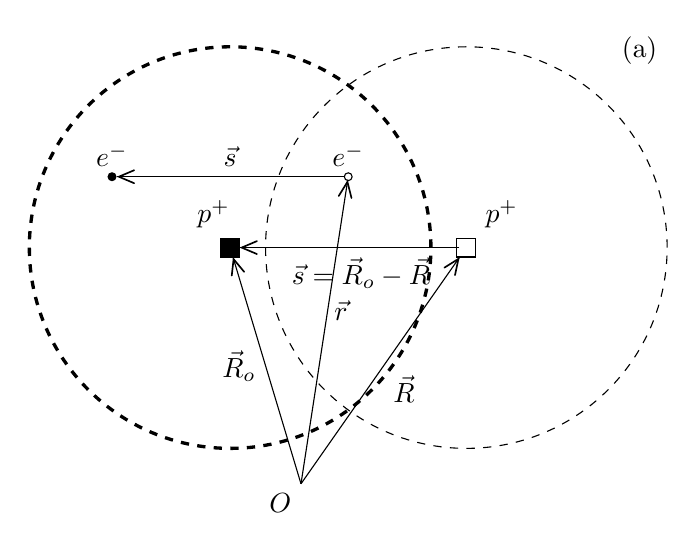
\begin{tikzpicture}
% define arrow head
[
    decoration={
      markings,
      mark=at position 1 with {\arrow[scale=1.5,black]{angle 45}};
    }
]

% scale
\pgfmathsetmacro{\a}{3}
\coordinate (H1) at (0,0);
\coordinate (H) at (\a,0);

% coordinate
\coordinate (O) at ($0.5*(H1)+0.3*(H)-(0,\a)$);
\node at (O) [below left]{$O$};

% ions
\pgfmathsetmacro{\R}{0.04*\a} % ion radius
\draw[fill] ($(H1)-(\R,\R)$) rectangle ($(H1)+(\R,\R)$) node [above left] {$p^+$};
\draw ($(H)-(\R,\R)$) rectangle ($(H)+(\R,\R)$) node [above right] {$p^+$};
\draw[postaction={decorate}] (O) -- ($0.96*(H)+0.04*(O)$);
\node at ($0.5*(H)+0.5*(O)$) [below right] {$\vec{R}$};
\draw[postaction={decorate}] (O) -- ($0.96*(H1)+0.04*(O)$);
\node at ($0.5*(H1)+0.5*(O)$) [left] {$\vec{R}_o$};

% wave function contour
\draw[very thick,dashed] (H1) circle (0.85*\a);
\draw[dashed] (H) circle (0.85*\a);

\coordinate (e) at (.5*\a,.3*\a);
\coordinate (e1) at ($(e)-(H)$);

% electrons
\node[draw,circle,inner sep=1pt] at (e) {};
\node at (e) [above] {$e^-$};
\node[draw,circle,inner sep=1pt,fill] at (e1) {};
\node at (e1) [above] {$e^-$};

% vectors
\draw[postaction={decorate}] (O) -- ($0.99*(e)+0.01*(O)$);
\node at ($0.5*(e)+0.5*(O)$) [above right] {$\vec{r}$};
\draw[postaction={decorate}] ($0.97*(H)$)--($0.04*(H)$);
\node at ($0.5*(H1)+0.22*(H)$) [below right] {$\vec{s}=\vec{R}_o-\vec{R}$};

\draw[postaction={decorate}] ($(e)-(0.02*\a,0)$) -- ($(e1)+(0.02*\a,0)$);
\node at ($0.5*(e)+0.5*(e1)$) [above] {$\vec{s}$};
%\draw[postaction={decorate}] (O) -- ($0.99*(e1)+0.01*(O)$);
%\node at ($0.5*(O)+0.5*(e1)$) [below left] {$\vec{r'}$};

% subplot marking
\node at (5.2,2.5) {(a)};

\end{tikzpicture}

\end{document}}
\subfloat[][$H_2^+$ molecule]{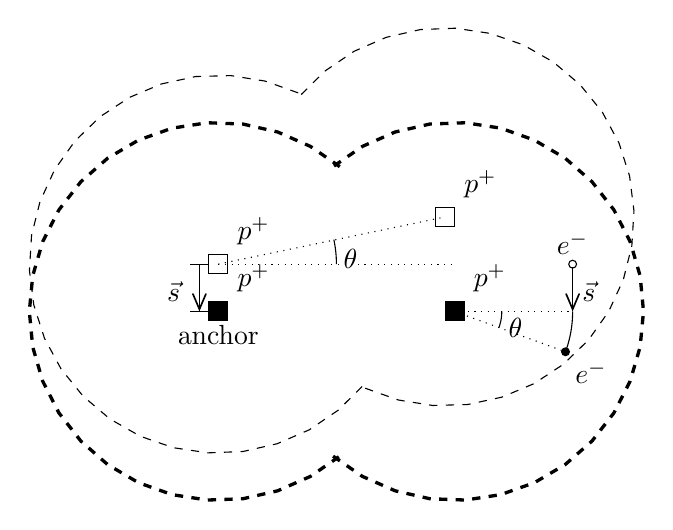
\begin{tikzpicture}
% define arrow head
[
    decoration={
      markings,
      mark=at position 1 with {\arrow[scale=1.5,black]{angle 45}};
    }
]
% scale
\pgfmathsetmacro{\a}{3}
\coordinate (H1) at (0,0);
\coordinate (H) at (\a,0);

% ions
\pgfmathsetmacro{\R}{0.04*\a} % ion radius
\draw[fill] ($(H1)-(\R,\R)$) rectangle ($(H1)+(\R,\R)$) node [above right] {$p^+$};
\draw[fill] ($(H)-(\R,\R)$) rectangle ($(H)+(\R,\R)$) node [above right] {$p^+$};
\draw [domain=50:310,dashed,very thick] plot ({0.8*\a*cos(\x)}, {0.8*\a*sin(\x)});
\draw [domain=-130:130,dashed,very thick] plot ({0.8*\a*cos(\x)+\a}, {0.8*\a*sin(\x)});
\node at ($(H1)-(0,0.1*\a)$) {anchor};

\pgfmathsetmacro{\s}{0.2*\a}
\draw[postaction={decorate}] ($(H1)+(-2*\R,\s)$) -- ($(H1)+(-2*\R,0)$);
\draw  ($(H1)+(-\R,\s)$) -- ($(H1)+(-3*\R,\s)$);
\draw  ($(H1)+(-\R,0)$) -- ($(H1)+(-3*\R,0)$) node [above left] {$\vec{s}$};
\coordinate (H1) at (0,\s);
\coordinate (H) at ($(\a-0.2*\s,2*\s)$);
% ions
\draw ($(H1)-(\R,\R)$) rectangle ($(H1)+(\R,\R)$) node [above right] {$p^+$};
\draw ($(H)-(\R,\R)$) rectangle ($(H)+(\R,\R)$) node [above right] {$p^+$};
\draw [domain=65:320,dashed] plot ({0.8*\a*cos(\x)}, {0.8*\a*sin(\x)+\s});
\draw [domain=-115:140,dashed] plot ({0.8*\a*cos(\x)+\a-0.2*\s}, {0.8*\a*sin(\x)+2*\s});

% electrons
\coordinate (e) at (1.5*\a,\s);
\node[draw,circle,inner sep=1pt] at (e) {};
\node at (e) [above] {$e^-$};
\draw[postaction={decorate}] ($(e)-(0,0.07*\s)$) -> ($(e)-(0,\s)$) node [above right] {$\vec{s}$};
\pgfmathsetmacro{\t}{20} % angle of electron
\coordinate (e1) at ({0.5*\a*cos(-\t)+\a}, {0.5*\a*sin(-\t)});
\draw [domain=0:-\t] plot ({0.5*\a*cos(\x)+\a}, {0.5*\a*sin(\x)});
\node[draw,circle,inner sep=1pt,fill] at (e1) {};
\node at (e1) [below right] {$e^-$};

% angle
\draw[dotted] (H1) -- (\a,\s); 
\draw[dotted] (H1) -- (H); 
\draw[dotted] (\a,0) -- ($(e)-(0,\s)$); 
\draw[dotted] (\a,0) -- ($(e1)$);
\draw[domain=0:12] plot ({0.5*\a*cos(\x)}, {0.5*\a*sin(\x)+\s}) node [below right] {$\theta$};
\draw[domain=0:-20] plot ({0.2*\a*cos(\x)+\a}, {0.2*\a*sin(\x)}) node [right] {$\theta$};
\end{tikzpicture}}
\caption{\textbf{Dragged Node Approximation} (a) For hydrogen atom, we assume the entire wavefunction shifts with the ion. This process can be visualized by following a contour of the wavefunction. The thick dashed circle represents a contour of the electron wavefunction when the proton is at its reference position $\vec{R}_o$ and the thin dashed circle represents the same contour when the proton has moved to a new position $\vec{R}$. To evaluate the ion-dependent electron wavefunction $\bar{\psi}_e(\vec{r},\vec{R})$, we simply map the electron to its proper place in the reference wavefunction. That is $\bar{\psi}_e(\vec{r},\vec{R})=\bar{\psi}_e(\vec{r}+\vec{s},\vec{R}_o)=\psi_e(\vec{r}+\vec{s})$ where $\vec{s}$ is the shift required to put the the proton back to its reference position. (b) For $H_2^+$, we pick one of the protons as an "anchor" and approximate the new wavefunction by dragging the reference wavefunction with the "anchor" proton. We also rotate the wavefunction to align its axis of symmetry with the orientation of the two protons. \label{fig:drag}  }
\end{figure*}

\section{Results and Discussion}
\subsection{Ionization Energies}
Ground state energies were calculated for first row atoms and ions with and without the adiabatic assumption (see Table \ref{tab:ionization}). The adiabatic ground state energies are in perfect agreement with previous QMC study \cite{Seth_Bench} and the ionization energies agree well with experimental results. It is interesting to note that even though ground state energies change significantly with the inclusion of non-adiabatic effects, the ionization energies match perfectly with or without the adiabatic assumption. This suggests that for atomic systems, non-adiabatic effects are indeed negligible. The difference in ground state energies can be entirely attributed to the zero point motion of the nucleus. 
\begin{table*}[htp!]
\setlength{\extrarowheight}{3pt}
\begin{tabular}{*{1}{*{8}{c}}}
\hline\hline
$\text{Atom}$ & $\text{Li}(^2\text{S)}$ & $\text{Be}(^1\text{S)}$ & $\text{B}(^2\text{P)}$ & $\text{C}(^3\text{P)}$ & $\text{N}(^4\text{S)}$ & $\text{O}(^3\text{P)}$ & $\text{F}(^2\text{P)}$ \\ \hline
$\text{Guess}$ & $\text{CAS(3,23)}$ & $\text{CAS(4,20)}$ & $\text{CAS(5,40)}$ & $\text{CAS(6,16)}$ & $\text{CAS(7,20)}$ & $\text{CAS(8,15)}$ & $\text{CAS(5,15)}$ \\
$\text{FN-DMCe}$ & $\text{-7.478056(4)}$ & $\text{-14.66731(1)}$ & $\text{-24.65377(1)}$ & $\text{-37.84451(2)}$ & $\text{-54.58851(3)}$ & $\text{-75.06554(4)}$ & $\text{-99.72286(7)}$ \\
$\text{FN-DMCe}_{\text{ref}}$ & $\text{-7.478067(5)}$ & $\text{-14.667306(7)}$ & $\text{-24.65379(3)}$ & $\text{-37.84446(6)}$ & $\text{-54.58867(8)}$ & $\text{-75.0654(1)}$ & $\text{-99.7318(1)}$ \\
$\text{FN-DMCei}$ & $\text{-7.47742(1)}$ & $\text{-14.66643(2)}$ & $\text{-24.65244(3)}$ & $\text{-37.84277(6)}$ & $\text{-54.58655(8)}$ & $\text{-75.0631(1)}$ & $\text{-99.7201(1)}$ \\
\hline
\end{tabular} \\ 
\begin{tabular}{*{1}{*{8}{c}}}
$\text{Ion}$ & $\text{Li+}(^1\text{S)}$ & $\text{Be+}(^2\text{S)}$ & $\text{B+}(^1\text{S)}$ & $\text{C+}(^2\text{P)}$ & $\text{N+}(^3\text{P)}$ & $\text{O+}(^4\text{S)}$ & $\text{F+}(^3\text{P)}$ \\ \hline
$\text{Guess}$ & $\text{CAS(2,5)}$ & $\text{CAS(3,18)}$ & $\text{CAS(4,40)}$ & $\text{CAS(5,16)}$ & $\text{CAS(6,20)}$ & $\text{CAS(5,15)}$ & $\text{CAS(4,15)}$ \\
$\text{FN-DMCe}$ & $0$ & $\text{-14.324753(6)}$ & $\text{-24.34884(1)}$ & $\text{-37.43075(2)}$ & $\text{-54.05376(3)}$ & $\text{-74.56588(4)}$ & $0$ \\
$\text{FN-DMCe}_{\text{ref}}$ & $\text{-7.279914(3)}$ & $\text{-14.324761(3)}$ & $\text{-24.34887(2)}$ & $\text{-37.43073(4)}$ & $\text{-54.05383(7)}$ & $\text{-74.56662(7)}$ & $\text{-99.0911(2)}$ \\
$\text{FN-DMCei}$ & $\text{}$ & $\text{-14.32386(2)}$ & $\text{-24.34750(3)}$ & $\text{-37.42904(4)}$ & $\text{-54.05182(9)}$ & $\text{-74.56336(8)}$ & $\text{}$ \\
\hline
$\text{IP}_{\text{e}}$  & 0 & 0.34256(2) & 0.3049(3) & 0.4138(5) & 0.53475(8) & 0.500(1) & 0 \\
$\text{IP}_{\text{ei}}$ & 0 & 0.34257(2) & 0.3049(3) & 0.4137(5) & 0.53473(8) & 0.500(1) & 0 \\
$\text{IP}_{\text{exp}}$ & 0.19808 & 0.3425 & 0.30502 & 0.413797 & 0.533967 & 0.500526 & 0.640173 \\
\hline
\end{tabular}
\caption{\textbf{Ionization Energies} Fixed-Node DMC was performed with and without the adiabatic assumption and the energies for each atom and ion is reported in units of Hartree. FN-DMCe denotes that only electrons are treated quantum mechanically while the ions are clamped in their equilibrium positions. FN-DMCei denotes that both electrons and ions are treated quantum mechanically. The reference is taken from \cite{Seth_Bench} \label{tab:ionization}}
\end{table*}
\subsection{Atomization Energies}
We also calculated ground state energies for LiH, LiH-, BeH and BH (see Table \ref{tab:atomization}). The energies calculated in the adiabatic limit are on par and sometimes better than the best available quantum chemistry results \cite{Adamowicz_LiH,Koput_BeH,Miliordos_BH} and the energies calculated without the adiabatic assumption are in excellent agreement with state-of-the-art quantum chemistry calculations performed with ECG. In the case of simple hydrides, non-adiabatic effects does make a noticeable contribution to the atomization energy 
\begin{table}[htp]
\setlength{\extrarowheight}{3pt}
\begin{tabular}{*{1}{*{5}{c}}}
\hline\hline
$\text{Molecule}$ & $\text{LiH}$ & $\text{LiH-}$ & $\text{BeH}$ & $\text{BH}$ \\ \hline
$\text{Guess}$ & $\text{CAS(4,43)}$ & $\text{CAS(5,17)}$ & $\text{CAS(5,44)}$ & $\text{CAS(4,14)}$ \\
$\text{FN-DMCe}$ & $\text{-8.070521(7)}$ & $\text{-8.08220(2)}$ & $\text{-15.24793(1)}$ & $\text{-25.28868(2)}$ \\
$E_{\text{Ref}}$ & $-8.07045$ & $0$ & $-15.247846$ & $-25.287650$ \\
$\text{FN-DMCei}$ & $\text{-8.06620(2)}$ & $\text{-8.07811(3)}$ & $\text{-15.24196(7)}$ & $\text{-25.28103(4)}$ \\
$\text{ECG}$ & $\text{-8.0664371(15)}$ & $-8.07856887$ & $\text{15.24203(10)}$ & $\text{-25.2803(10)}$ \\ \hline
$E^{\text{at}}_{e}$ & 0.092465(8)& N/A & 0.08062(1) & 0.13491(2) \\
$E^{\text{at}}_{ei}$ & 0.08888(2)& N/A & 0.07563(7) & 0.12869(5) \\
$E^{\text{at}}_{\text{ref}}$ & 0.08937(5) & N/A & 0.0761(4) & 0.1298(2) \\
$E^{\text{at}}_{\text{exp}}$ & 0.08874(38) & N/A & 0.0826(11) & 0.1281(37) \\
\hline\hline
\end{tabular}
\caption{\textbf{Atomization Energies} $E^{\text{at}}_{e}$ is the atomization energy in the adiabatic limit, whereas $E^{\text{at}}_{ei}$ is obtained without the adiabatic assumption. $E^{\text{at}}_{\text{ref}}$ is taken from \cite{Feller_Corrections} and $E^{\text{at}}_{\text{exp}}$ is obtained from \cite{CCCBDB} \label{tab:atomization}}
\end{table} 


\pagebreak
\bibliographystyle{unsrt}
\bibliography{ref}
\end{document}